%beamer

% Define a global usable date. Must come before StyleTut
% \newcommand{\mydate}{09.12.2016}

% Comment/uncomment this line to toggle handout mode
% \newcommand{\handout}{}

%% Beamer-Klasse im korrekten Modus
\ifdefined \handout
\documentclass[handout]{beamer} % Handout mode
\else
\documentclass{beamer}
\fi

%% UTF-8-Encoding
\usepackage[utf8]{inputenc}

% % \bigtimes abgeschrieben von http://tex.stackexchange.com/questions/14386/importing-a-single-symbol-from-a-different-font
% \DeclareFontFamily{U}{mathx}{\hyphenchar\font45}
% \DeclareFontShape{U}{mathx}{m}{n}{
%       <5> <6> <7> <8> <9> <10> gen * mathx
%       <10.95> mathx10 <12> <14.4> <17.28> <20.74> <24.88> mathx12
%       }{}
% \DeclareSymbolFont{mathx}{U}{mathx}{m}{n}
% \DeclareMathSymbol{\bigtimes}{\mathop}{mathx}{161}

\RequirePackage{xcolor}

\def\9{\square}
%\def\9{\blank}

% f"ur Aussagenlogik
\colorlet{alcolor}{blue}
\RequirePackage{tikz}
\usetikzlibrary{arrows.meta}
\newcommand{\alimpl}{\mathrel{\tikz[x={(0.1ex,0ex)},y={(0ex,0.1ex)},>={Classical TikZ Rightarrow[]}]{\draw[alcolor,->,line width=0.7pt,line cap=round] (0,0) -- (15,0);\path (0,-6);}}}
\newcommand{\aleqv}{\mathrel{\tikz[x={(0.1ex,0ex)},y={(0ex,0.1ex)},>={Classical TikZ Rightarrow[]}]{\draw[alcolor,<->,line width=0.7pt,line cap=round] (0,0) -- (18,0);\path (0,-6);}}}
\newcommand{\aland}{\mathbin{\raisebox{-0.6pt}{\rotatebox{90}{\texttt{\color{alcolor}\char62}}}}}
\newcommand{\alor}{\mathbin{\raisebox{-0.8pt}{\rotatebox{90}{\texttt{\color{alcolor}\char60}}}}}
%\newcommand{\ali}[1]{_{\mathtt{\color{alcolor}#1}}}
\newcommand{\alv}[1]{\mathtt{\color{alcolor}#1}}
\newcommand{\alnot}{\mathop{\tikz[x={(0.1ex,0ex)},y={(0ex,0.1ex)}]{\draw[alcolor,line width=0.7pt,line cap=round,line join=round] (0,0) -- (10,0) -- (10,-4);\path (0,-8) ;}}}
\newcommand{\alP}{\alv{P}} %ali{#1}}
%\newcommand{\alka}{\negthinspace\hbox{\texttt{\color{alcolor}(}}}
\newcommand{\alka}{\negthinspace\text{\texttt{\color{alcolor}(}}}
%\newcommand{\alkz}{\texttt{\color{alcolor})}}\negthinspace}
\newcommand{\alkz}{\text{\texttt{\color{alcolor})}}\negthinspace}
\newcommand{\AAL}{A_{AL}}
\newcommand{\LAL}{\hbox{\textit{For}}_{AL}}
\newcommand{\AxAL}{\hbox{\textit{Ax}}_{AL}}
\newcommand{\AxEq}{\hbox{\textit{Ax}}_{Eq}}
\newcommand{\AxPL}{\hbox{\textit{Ax}}_{PL}}
\newcommand{\AALV}{\hbox{\textit{Var}}_{AL}}
\newcommand{\MP}{\hbox{\textit{MP}}}
\newcommand{\GEN}{\hbox{\textit{GEN}}}
\newcommand{\W}{\ensuremath{\hbox{\textbf{w}}}\xspace}
\newcommand{\F}{\ensuremath{\hbox{\textbf{f}}}\xspace}
\newcommand{\WF}{\ensuremath{\{\W,\F\}}\xspace}
\newcommand{\val}{\hbox{\textit{val}}}
\newcommand{\valDIb}{\val_{D,I,\beta}}

\newcommand*{\from}{\colon}

% die nachfolgenden Sachen angepasst an cmtt
\newlength{\ttquantwd}
\setlength{\ttquantwd}{1ex}
\newlength{\ttquantht}
\setlength{\ttquantht}{6.75pt}
\def\plall{%
  \tikz[line width=0.67pt,line cap=round,line join=round,baseline=(B),alcolor] {
    \draw (-0.5\ttquantwd,\ttquantht) -- node[coordinate,pos=0.4] (lll){} (-0.25pt,-0.0pt) -- (0.25pt,-0.0pt) -- node[coordinate,pos=0.6] (rrr){} (0.5\ttquantwd,\ttquantht);
    \draw (lll) -- (rrr);
    \coordinate (B) at (0,-0.35pt);
  }%
}
\def\plexist{%
  \tikz[line width=0.67pt,line cap=round,line join=round,baseline=(B),alcolor] {
    \draw (-0.9\ttquantwd,\ttquantht) -- (0,\ttquantht) -- node[coordinate,pos=0.5] (mmm){} (0,0) --  (-0.9\ttquantwd,0);
    \draw (mmm) -- ++(-0.75\ttquantwd,0);
    \coordinate (B) at (0,-0.35pt);
  }\ensuremath{\,}%
}
\let\plexists=\plexist
\newcommand{\NT}[1]{\ensuremath{\langle\mathrm{#1} \rangle}}

\newcommand{\CPL}{\text{\itshape Const}_{PL}}
\newcommand{\FPL}{\text{\itshape Fun}_{PL}}
\newcommand{\RPL}{\text{\itshape Rel}_{PL}}
\newcommand{\VPL}{\text{\itshape Var}_{PL}}
\newcommand{\ATer}{A_{\text{\itshape Ter}}}
\newcommand{\ARel}{A_{\text{\itshape Rel}}}
\newcommand{\AFor}{A_{\text{\itshape For}}}
\newcommand{\LTer}{L_{\text{\itshape Ter}}}
\newcommand{\LRel}{L_{\text{\itshape Rel}}}
\newcommand{\LFor}{L_{\text{\itshape For}}}
\newcommand{\NTer}{N_{\text{\itshape Ter}}}
\newcommand{\NRel}{N_{\text{\itshape Rel}}}
\newcommand{\NFor}{N_{\text{\itshape For}}}
\newcommand{\PTer}{P_{\text{\itshape Ter}}}
\newcommand{\PRel}{P_{\text{\itshape Rel}}}
\newcommand{\PFor}{P_{\text{\itshape For}}}

\newcommand{\plka}{\alka}
\newcommand{\plkz}{\alkz}
%\newcommand{\plka}{\plfoo{(}}
%\newcommand{\plkz}{\plfoo{)}}
\newcommand{\plcomma}{\hbox{\texttt{\color{alcolor},}}}
\newcommand{\pleq}{{\color{alcolor}\,\dot=\,}}

% MODIFIED (DJ)
% previously: \newcommand{\plfoo}[1]{\mathtt{\color{alcolor}#1}}
\newcommand{\plfoo}[1]{\texttt{\color{alcolor}#1}}

\newcommand{\plc}{\plfoo{c}}
\newcommand{\pld}{\plfoo{d}}
\newcommand{\plf}{\plfoo{f}}
\newcommand{\plg}{\plfoo{g}}
\newcommand{\plh}{\plfoo{h}}
\newcommand{\plx}{\plfoo{x}}
\newcommand{\ply}{\plfoo{y}}
\newcommand{\plz}{\plfoo{z}}
\newcommand{\plR}{\plfoo{R}}
\newcommand{\plS}{\plfoo{S}}

\newcommand{\bv}{\mathrm{bv}}
\newcommand{\fv}{\mathrm{fv}}

%\newcommand{\AxAL}{\hbox{\textit{Ax}}_{AL}}
%\newcommand{\AALV}{\hbox{\textit{Var}}_{AL}}

%\renewcommand{\#}[1]{\literal{#1}}
\newcommand{\A}{\mathcal{A}}
\newcommand{\Adr}{\text{Adr}}
\newcommand{\ar}{\mathrm{ar}}
\newcommand{\ascii}[1]{\literal{\char#1}}
%\newcommand{\assert}[1]{\text{/\!\!/\ } #1}
\newcommand{\assert}[1]{\colorbox{black!7!white}{\ensuremath{\{\;#1\;\}}}}
\newcommand{\Assert}[1]{$\langle$\textit{#1}$\rangle$}
\newcommand{\B}{\mathcal{B}}
\newcommand{\bfmod}{\mathbin{\kw{ mod }}}
\newcommand{\bb}{{\text{bb}}}
\def\bottom{\hbox{\small$\pmb{\bot}$}}
\newcommand{\card}[1]{|#1|}
%\newcommand{\cod}{\mathop{\text{cod}}}  % ist in thwmathabbrevs
\newcommand{\Conf}{\mathcal{C}}
\newcommand{\define}[1]{\emph{#1}}
%\renewcommand{\dh}{d.\,h.\@\xspace}
%\newcommand{\Dh}{D.\,h.\@\xspace}
%\newcommand{\engl}[1]{engl.\xspace\emph{#1}}
\newcommand{\eps}{\varepsilon}
%\newcommand{\evtl}{evtl.\@\xspace}
\newcommand{\fbin}{\text{bin}}
\newcommand{\finv}{\text{inv}}
\newcommand{\fnum}{\text{num}}
\newcommand{\fNum}{{\text{Num}}}
\newcommand{\frepr}{\text{repr}}
\newcommand{\fRepr}{\text{Repr}}
\newcommand{\fZkpl}{\text{Zkpl}}
\newcommand{\fLen}{\text{Len}}
\newcommand{\fsem}{\text{sem}}
\providecommand{\fspace}{\mathord{\text{space}}}
\providecommand{\fSpace}{\mathord{\text{Space}}}
\providecommand{\ftime}{\mathord{\text{time}}}
\providecommand{\fTime}{\mathord{\text{Time}}}
\newcommand{\fTrans}{\text{Trans}}
\newcommand{\fVal}{\text{Val}}

% Modified (DJ)
\newcommand{\Val}{\text{Val}}

%\def\G{\mathbb{Z}}
\newcommand{\HT}[1]{\normalfont\textsc{HT-#1}}
\newcommand{\htr}[3]{\{#1\}\;#2\; \{#3\}}
\newcommand{\Id}{\text{I}}
%\newcommand{\ie}{i.\,e.\@\xspace}
\newcommand{\instr}[2]{\texttt{#1}\ \textit{#2}}
\newcommand{\Instr}[2]{\texttt{#1}\ \textrm{#2}}
\newcommand{\instrr}[3]{\texttt{#1}\ \textit{#2}\texttt{(#3)}}
\newcommand{\Instrr}[3]{\texttt{#1}\ \textrm{#2}\texttt{(#3)}}
\newcommand{\io}{\!\mid\!}
\usepackage{KITcolors}
\newcommand{\literal}[1]{\hbox{\textcolor{blue!95!white}{\textup{\texttt{\scalebox{1.11}{#1}}}}}}
%\newcommand{\literal}[1]{\hbox{\textcolor{KITblue!80!black}{\textup{\texttt{#1}}}}}
\def\kasten#1{\leavevmode\literal{\setlength{\fboxsep}{1pt}\fbox{\vrule  width 0pt height 1.5ex depth 0.5ex #1}}}
\newcommand{\kw}[1]{\ensuremath{\mathbf{#1}}}
\newcommand{\lang}[1]{\ensuremath{\langle#1\rangle}}
%\newcommand{\maw}{m.\,a.\,w.\@\xspace}
%\newcommand{\MaW}{M.\,a.\,w.\@\xspace}
\newcommand{\mdefine}[2][FOOBAR]{\define{#2}\def\foobar{FOOBAR}\def\optarg{#1}\ifx\foobar\optarg\def\optarg{#2}\fi\graffito{\optarg}}
\newcommand{\meins}{\rotatebox[origin=c]{180}{1}}
\newcommand{\Mem}{\text{Mem}}
\newcommand{\memread}{\text{memread}}
\newcommand{\memwrite}{\text{memwrite}}
\providecommand{\meta}[1]{\ensuremath{\langle}\textit{#1}\ensuremath{\rangle}}
%\newcommand{\N}{\mathbb{N}}
\newcommand{\NP}{\mathbf{NP}}
\newcommand{\Nadd}{N_{\text{add}}}
\newcommand{\Nmult}{N_{\text{mult}}}
\newcommand{\Oh}[1]{O\left(#1\right)}
\newcommand{\Om}[1]{\Omega\left(#1\right)}
\newcommand{\personname}[1]{\textsc{#1}}
\newcommand{\regname}[1]{\texttt{#1}}
\newcommand{\mima}{\textsc{Mima}\xspace}
\newcommand{\mimax}{\textsc{Mima-X}\xspace}

\def\Pclass{\text{\bfseries P}}
\def\PSPACE{\text{\bfseries PSPACE}}

\newcommand{\SPush}{\text{push}}
\newcommand{\SPop}{\text{pop}}
\newcommand{\SPeek}{\text{peek}}
\newcommand{\STop}{\text{top}}
\newcommand{\STos}{\text{\itshape tos}}
\newcommand{\SBos}{\text{\itshape bos}}

%\newcommand{\R}{\mathbb{R}}
\newcommand{\Rnullplus}{\R_0^{+}}
\newcommand{\Rplus}{\R_{+}}
\newcommand{\resp}{resp.\@\xspace}
\newcommand{\Sem}{\text{Sem}}
\newcommand{\sgn}{\mathop{\text{sgn}}}
\newcommand{\sqbox}{\mathop{\raisebox{-6.2pt}{\hbox{\hbox to 0pt{$^{^{\sqcap}}$\hss}$^{^{\sqcup}}$}}}}
\newcommand{\sqleq}{\sqsubseteq}
\newcommand{\sqgeq}{\sqsupseteq}
\newcommand{\Th}[1]{\Theta\left(#1\right)}
%\newcommand{\usw}{usw.\@\xspace}
\newcommand{\V}[1]{\hbox{\textit{#1}}}
\newcommand{\x}{\times}
\newcommand{\ZK}{\mathbb{K}}
%\newcommand{\Z}{\mathbb{Z}}
%\newcommand{\zB}{z.\,B.\@\xspace}
%\newcommand{\ZB}{Z.\,B.\@\xspace}
% \newcommand{\bb}{{\text{bb}}}
% \def\##1{\hbox{\textcolor{darkblue}{\texttt{#1}}}}
% \def\A{\mathcal{A}}
% \newcommand{\0}{\#0}
% \newcommand{\1}{\#1}
% \newcommand{\Obj}{\text{Obj}}
% \newcommand{\start}{\mathop{\text{start}}}
% \newcommand{\compactlist}{\addtolength{\itemsep}{-\parskip}}
% \newcommand{\fval}{\text{val}}
% \newcommand{\lang}[1]{\ensuremath{\langle#1\rangle}}
% \newcommand{\io}{\!\mid\!}
% \def\sqbox{\mathop{\raisebox{-6.2pt}{\hbox{\hbox to 0pt{$^{^{\sqcap}}$\hss}$^{^{\sqcup}}$}}}}
% \def\sqleq{\sqsubseteq}
% \def\sqgeq{\sqsupseteq}
\def\Td{T_{\overline{d}}}
% \newcommand{\csym}[1]{\ensuremath{\#{c}_{\#{\hbox{\scriptsize #1}}}}}
% \newcommand{\F}{\ensuremath{\mathcal{F}}}
% \newcommand{\fsym}[2]{\ensuremath{\#{f}^{\#{\hbox{\scriptsize #1}}}_{\#{\hbox{\scriptsize #2}}}}}
% \newcommand{\rsym}[2]{\ensuremath{\#{R}^{\#{\hbox{\scriptsize #1}}}_{\#{\hbox{\scriptsize #2}}}}}
% \newcommand{\xsym}[1]{\ensuremath{\#{x}_{\#{\hbox{\scriptsize #1}}}}}
% \newcommand{\I}{\mathcal{I}}
% ********************************************************************

\usepackage{../TutTexbib/thwregex}
\usepackage{environ}
\usepackage{bm}
\usepackage{calc}
\usepackage{varwidth}
\usepackage{wasysym}
\usepackage{mathtools}

%% Tabellen
\usepackage{array}
\usepackage{multicol}

%% Bibliotheken für viele mathematische Symbole
\usepackage{amsmath, amsfonts, amssymb}



% This is a configuration file with personal tutor information.
% It is therefore excluded from the git repository, so changes in this file will not conflict in git commits.

% Copy this template, rename to config.tex and add your information below.

\newcommand{\myname}{Lukas Morawietz}
\newcommand{\mymail}{lukas.morawietz@gmail.com} % Consider using your named student mail address to keep your u**** account private.
\newcommand{\mytutnumber}{31}

% Don't forget to update ILIAS url. WARNING: Underscores '_' and Ampersands '&' have to be escaped with backslashes '\'. Blame TeX, not me.
\newcommand{\myILIASurl}{https://ilias.studium.kit.edu/ilias.php?ref\_id=855240\&cmdClass=ilrepositorygui\&cmdNode=5r\&baseClass=ilrepositorygui}

% Uncommenting this will print Socrative info with here defined roomname whenever \Socrative is called.
% (Otherwise, \Socrative will remain silent.)
% \newcommand{\mysocrativeroom}{???}

%\def\ThassesTut{}
\def\DanielsTut{}

\newcommand{\aboutMeFrame}{
	\begin{frame}{Über mich}
		\myname \\
		Informatik, 9. Fachsemester (Bachelor)
		% Lebensgeschichte...
		% Stammbaum...
		% Aufarbeitung der eigenen Todesser-Vergangenheit...
	\end{frame}
}

\def\thisyear{2019}

% Update date of exam
\def\myKlausurtermin{18.~März~2020, 14:00–16:00~Uhr}

\def\mydate#1{
		  \ifnum#1=1\relax	  23. Oktober \thisyear \
	\else \ifnum#1=2\relax	  30. Oktober \thisyear \
	\else \ifnum#1=3\relax    06. November \thisyear \
	\else \ifnum#1=4\relax    13. November \thisyear \
	\else \ifnum#1=5\relax    20. November \thisyear \
	\else \ifnum#1=6\relax    27. November \thisyear \
	\else \ifnum#1=7\relax    04. Dezember \thisyear \
	\else \ifnum#1=8\relax    11. Dezember \thisyear \
	\else \ifnum#1=9\relax    18. Dezember \thisyear \
	\else \ifnum#1=10\relax   08. Januar \nextyear \
	\else \ifnum#1=11\relax   15. Januar \nextyear \
	\else \ifnum#1=12\relax   22. Januar \nextyear \
	\else \ifnum#1=13\relax   29. Januar \nextyear \
	\else \ifnum#1=14\relax   05. Februar \nextyear \
	\else \textbf{Datum undefiniert!} 
	\fi\fi\fi\fi\fi\fi\fi\fi\fi\fi\fi\fi\fi\fi
}

\def\mylasttimestext{Was letztes Mal geschah...}

\colorlet{beamerlightred}{red!40}
\colorlet{beamerlightgreen}{green!50}
\colorlet{beamerlightyellow}{yellow!50}
\colorlet{lightred}{red!30}
\colorlet{lightgreen}{green!40}
\colorlet{lightyellow}{yellow!50}
\colorlet{fullred}{red!60}
\colorlet{fullgreen}{green}

\definecolor{myalertcolor}{rgb}{1,0.33,0.24}
\setbeamercolor{alerted text}{fg=myalertcolor}

% Flag to toggle display of KIT Logo.
% If you want to conform to the official logo guidelines, 
% you are not allowed to use the logo and should disable it
% using the following flag. Just saying.
% (But it's too beautiful, so best leave this commented. :P)
%\newcommand{\noKITLogo}{}

% Toggle handout mode by including the following line before including PraeambelTut
% and removing the % at the start (but do NOT remove the % char here, otherwise handout mode will always be on!)
% Please keep handout mode off in all commits!

% \newcommand{\handout}{}



% define custom \handout command flag if handout mode is toggled  #DirtyAsHellButWell...
\only<beamer:0>{\def\handout{}} %beamer:0 == handout mode

\newcommand{\R}{\mathbb{R}}
\newcommand{\N}{\mathbb{N}}
\newcommand{\Z}{\mathbb{Z}}
\newcommand{\Q}{\mathbb{Q}}
\newcommand{\BB}{\mathbb{B}}
\newcommand{\C}{\mathbb{C}}
\newcommand{\K}{\mathbb{K}}
\newcommand{\G}{\mathbb{G}}
\newcommand{\nullel}{\mathcal{O}}
\newcommand{\einsel}{\mathds{1}}
\newcommand{\Pot}{\mathcal{P}}
\renewcommand{\O}{\text{O}}

\def\word#1{\hbox{\textcolor{blue}{\texttt{#1}}}}
\let\literal\word
\def\mword#1{\hbox{\textcolor{blue}{$\mathtt{#1}$}}}  % math word
\def\sp{\scalebox{1}[.5]{\textvisiblespace}}
\def\wordsp{\word{\sp}}

%\newcommand{\literal}[1]{\textcolor{blue}{\texttt{#1}}}
\newcommand{\realTilde}{\textasciitilde \ }
\newcommand{\setsize}[1]{\ensuremath{\left\lvert #1 \right\rvert}}
\let\size\setsize
\newcommand{\set}[1]{\left\{#1\right\}}
\newcommand{\tuple}[1]{\left(#1\right)}
\newcommand{\normalvar}[1]{\text{$#1$}}

% Modified by DJ
\let\oldemptyset\emptyset
\let\emptyset\varnothing % proper emptyset

%\definecolor{myRed}{RGB}{255,75,20}
%\colorlet{myGreen}{KITpalegreen}

%\newcounter{tfqtempcount}
%\newcommand{\truefalseQ}[4]{
%	\setcounter{tfqtempcount}{#1}
%	\addtocounter{tfqtempcount}{1}
%	\truefalseQuestion{#1}{\value{tfqtempcount}}{#2}{#3}{#4}
%}

%\newcommand{\truefalseQuestion}[5]{\item<#1-|handout:#1-> \color<#2-|handout:#2->{#3} #4 \qquad \visible<#2-|handout:#2->{#5}}

\newcommand{\boder}{\ensuremath{\mathbin{\textcolor{blue}{\vee}}}\xspace}
\newcommand{\bund}{\ensuremath{\mathbin{\textcolor{blue}{\wedge}}}\xspace}
\newcommand{\bimp}{\ensuremath{\mathrel{\textcolor{blue}{\to}}}\xspace}
\newcommand{\bgdw}{\ensuremath{\mathrel{\textcolor{blue}{\leftrightarrow}}}\xspace}
\newcommand{\bnot}{\ensuremath{\textcolor{blue}{\neg}}\xspace}
\newcommand{\bone}{\ensuremath{\textcolor{blue}{1}}\text{}}
\newcommand{\bzero}{\ensuremath{\textcolor{blue}{0}}\text{}}
\newcommand{\bleftBr}{\ensuremath{\textcolor{blue}{\texttt{(}}}\text{}}
\newcommand{\brightBr}{\ensuremath{\textcolor{blue}{\texttt{)}}}\text{}}

\newcommand{\plB}{\plfoo{B}}
\newcommand{\plE}{\plfoo{E}}

\newcommand{\summe}[2]{\sum\limits_{#1}^{#2}}
\newcommand{\limes}[1]{\lim\limits_{#1}}

%\newcommand{\numpp}{\advance \value{weeknum} by -2 \theweeknum \advance \value{weeknum} by 2}
%\newcommand{\nump}{\advance \value{weeknum} by -1 \theweeknum \advance \value{weeknum} by 1}

\newcommand{\mycomment}[1]{}
\newcommand{\Comment}[1]{}

%% DISCLAIMER START 
% It is INSANELY IMPORTANT NOT TO DO THIS OUTSIDE BEAMER CLASS! IN ARTCILE DOCUMENTS, THIS IS VERY LIKELY TO BUG AROUND!
\makeatletter%
\@ifclassloaded{beamer}%
{
	% TODO 
	% no time...
	% redefine section to ignore multiple \section calls with the same title
}%
{
	\errmessage{ERROR: section command redefinition outside of beamer class document! Please contact the author of this code.}
}%
\makeatother%
%% DISCLAIMER END

\newcounter{abc}
\newenvironment{alist}{
  \begin{list}{(\alph{abc})}{
      \usecounter{abc}\setlength{\leftmargin}{8mm}\setlength{\labelsep}{2mm}
    }
}{\end{list}}


\newcommand{\stdarraystretch}{1.20}
\renewcommand{\arraystretch}{\stdarraystretch}  % for proper row spacing in tables

\newcommand{\morescalingdelimiters}{   % for proper \left( \right) typography
	\delimitershortfall=-1pt  
	\delimiterfactor=1
}

\newcommand{\centered}[1]{\vspace{-\baselineskip}\begin{center}#1\end{center}\vspace{-\baselineskip}}

% for \implitem and \item[bla] stuff to look right:
\setbeamercolor*{itemize item}{fg=black}
\setbeamercolor*{itemize subitem}{fg=black}
\setbeamercolor*{itemize subsubitem}{fg=black}

\setbeamercolor*{description item}{fg=black}
\setbeamercolor*{description subitem}{fg=black}
\setbeamercolor*{description subsubitem}{fg=black}

\renewcommand{\qedsymbol}{\textcolor{black}{\openbox}}

\renewcommand{\mod}{\mathop{\textbf{mod}}}
\renewcommand{\div}{\mathop{\textbf{div}}}

\newcommand{\ceil}[1]{\left\lceil#1\right\rceil}
\newcommand{\floor}[1]{\left\lfloor#1\right\rfloor}
\newcommand{\abs}[1]{\left\lvert #1 \right\rvert}
\newcommand{\Matrix}[1]{\begin{pmatrix} #1 \end{pmatrix}}
\newcommand{\braced}[1]{\left\lbrace #1 \right\rbrace}

\def\fract#1/#2 {\frac{#1}{#2}} % ! Trailing space is crucial!
\def\dfract#1/#2 {\dfrac{#1}{#2}} % ! Trailing space is crucial!

\newcommand{\Mid}{\;\middle|\;}

\let\after\circ

\def\·{\cdot}
\def\*{\cdot}
\def\?>{\ensuremath{\rightsquigarrow}}  % Fuck you, Latex

\newcommand{\tight}[1]{{\renewcommand{\arraystretch}{0.76} #1}}
\newcommand{\stackedtight}[1]{{\renewcommand{\arraystretch}{0.76} \begin{matrix} #1 \end{matrix}} }
\newcommand{\stacked}[1]{\begin{matrix} #1 \end{matrix} }
\newcommand{\casesl}[1]{\delimitershortfall=0pt  \left\lbrace\hspace{-.3\baselineskip}\begin{array}{ll} #1 \end{array}\right.}
\newcommand{\casesr}[1]{\delimitershortfall=0pt  \left.\begin{array}{ll} #1 \end{array}\hspace{-.3\baselineskip}\right\rbrace}
\newcommand{\caseslr}[1]{\delimitershortfall=0pt  \left\lbrace\hspace{-.3\baselineskip}\begin{array}{ll} #1 \end{array}\hspace{-.3\baselineskip}\right\rbrace}

\def\q#1uad{\ifnum#1=0\relax\else\quad\q{\the\numexpr#1-1\relax}uad\fi}
% e.g. \q1uad = \quad, \q2uad = \qquad etc.

\newcommand{\qqquad}{\q3uad}

\newcommand{\impl}{\ifmmode\ensuremath{\mskip\thinmuskip\Rightarrow\mskip\thinmuskip}\else$\Rightarrow$\fi\xspace}
\newcommand{\Impl}{\ifmmode\implies\else$\Longrightarrow$\fi\xspace}

\newcommand{\derives}{\Rightarrow}

\newcommand{\gdw}{\ifmmode\mskip\thickmuskip\Leftrightarrow\mskip\thickmuskip\else$\Leftrightarrow$\fi\xspace}
\newcommand{\Gdw}{\ifmmode\iff\else$\Longleftrightarrow$\fi\xspace}

\newcommand{\symbitemnegoffset}{\hspace{-.5\baselineskip}}
\newcommand{\implitem}{\item[\impl\symbitemnegoffset]}
\newcommand{\Implitem}{\item[\Impl\symbitemnegoffset]}


\newcommand{\forcenewline}{\mbox{}\\}


% proper math typography
\newcommand{\functionto}{\longrightarrow}
\renewcommand{\geq}{\geqslant}
\renewcommand{\leq}{\leqslant}
\let\oldsubset\subset
\renewcommand{\subset}{\subseteq} % for all idiots out there using subset

\newenvironment{threealign}{%
	\[
	\begin{array}{r@{\ }c@{\ }l}
}{%
	\end{array}	
	\]
}

\newcommand{\concludes}{ \\ \hline  }
\newcommand{\deduction}[1]{
	\begin{varwidth}{.8\linewidth}
		\begin{tabular}{>{$}c<{$}}
			#1
		\end{tabular}
	\end{varwidth}	
}

\definecolor{hoareorange}{rgb}{1,.85,.6}
\newcommand{\hoareassert}[1]{\setlength{\fboxsep}{1pt}\setlength{\fboxrule}{-1.4pt}\fcolorbox{white}{hoareorange}{\ensuremath{\{\;#1\;\}}}\setlength\fboxrule{\defaultfboxrule}\setlength{\fboxsep}{3pt}}

\newcommand{\mailto}[1]{\href{mailto:#1}{{\textcolor{blue}{\underline{#1}}}}}
\newcommand{\urlnamed}[2]{\href{#2}{\textcolor{blue}{\underline{#1}}}}
\renewcommand{\url}[1]{\urlnamed{#1}{#1}}

\newcommand{\hanging}{\hangindent=0.7cm}
\newcommand{\indented}{\hanging}

%requires \thisyear to be defined (s. config.tex)!
\edef\nextyear{\the\numexpr\thisyear+1\relax}


% --- \frameheight constant ---
\newlength\fullframeheight
\newlength\framewithtitleheight
\setlength\fullframeheight{.92\textheight}
\setlength\framewithtitleheight{.86\textheight}

\newlength\frameheight
\setlength\frameheight{\fullframeheight}

\let\frametitleentry\relax
\let\oldframetitle\frametitle
\def\newframetitle#1{\global\def\frametitleentry{#1}\if\relax\frametitleentry\relax\else\setlength\frameheight{\framewithtitleheight}\fi\oldframetitle{#1}}
\let\frametitle\newframetitle

\def\newframetitleoff{\let\frametitle\oldframetitle}
\def\newframetitleon{\let\frametitle\newframetitle}
% --- \frameheight constant end ---



\newenvironment{headframe}{\Huge THIS IS AN ERROR. PLEASE CONTACT THE ADMIN OF THIS TEX CODE. (headframe env def failed)}{}
\RenewEnviron{headframe}[1][]{
	\begin{frame}\frametitle{\ }
		\centering
		\Huge\textbf{\textsc{\BODY} \\
		}
		\Large {#1}
		\frametitle{\ }
	\end{frame}
}


\makeatletter
% Provides color if undefined.
\newcommand{\colorprovide}[2]{%
	\@ifundefinedcolor{#1}{\colorlet{#1}{#2}}{}}
\makeatother


\colorprovide{lightred}{red!30}
\colorprovide{lightgreen}{green!40}
\colorprovide{lightyellow}{yellow!50}
\colorprovide{beamerlightred}{lightred}
\colorprovide{beamerlightgreen}{lightgreen}
\colorprovide{beamerlightyellow}{lightyellow}
\colorprovide{fullred}{red!60}
\colorprovide{fullgreen}{green}
\definecolor{darkred}{RGB}{115,48,38}
\definecolor{darkgreen}{RGB}{48,115,38}
\definecolor{darkyellow}{RGB}{100,100,0}

\only<handout:0>{\colorlet{adaptinglightred}{beamerlightred}}
\only<handout:0>{\colorlet{adaptinglightgreen}{beamerlightgreen}}
\only<handout:0>{\colorlet{adaptinglightred}{beamerlightred}}
\only<beamer:0>{\colorlet{adaptinglightred}{lightred}}
\only<beamer:0>{\colorlet{adaptinglightgreen}{lightgreen}}
\only<beamer:0>{\colorlet{adaptinglightred}{lightred}}
\only<handout:0>{\colorlet{adaptingred}{lightred}}
\only<beamer:0>{\colorlet{adaptingred}{fullred}}
\only<handout:0>{\colorlet{adaptinggreen}{lightgreen}}
\only<beamer:0>{\colorlet{adaptinggreen}{fullgreen}}



\newcommand{\TrueQuestion}[1]{
	\TrueQuestionE{#1}{}
}

\newcommand{\YesQuestion}[1]{
	\YesQuestionE{#1}{}
}

\newcommand{\FalseQuestion}[1]{
	\FalseQuestionE{#1}{}
}

\newcommand{\NoQuestion}[1]{
	\NoQuestionE{#1}{}
}

\newcommand{\DependsQuestion}[1]{
	\DependsQuestionE{#1}{}
}

\newcommand{\QuestionVspace}{\vspace{4pt}}
\newcommand{\QuestionParbox}[1]{\begin{varwidth}{.85\linewidth}#1\end{varwidth}}
\newcommand{\ExplanationParbox}[1]{\begin{varwidth}{.97\linewidth}#1\end{varwidth}}
\colorlet{questionlightgray}{gray!23}
\let\defaultfboxrule\fboxrule

% #1: bg color
% #2: fg color short answer
% #3: short answer text
% #4: question
% #5: explanation
\newcommand{\GenericQuestion}[5]{
	\setlength\fboxrule{2pt}
	\only<+|handout:0>{\hspace{-2pt}\fcolorbox{white}{questionlightgray}{\QuestionParbox{#4} \quad\textbf{?}}}
	\visible<+->{\hspace{-2pt}\fcolorbox{white}{#1}{\QuestionParbox{#4} \quad\textbf{\textcolor{#2}{#3}}} \ExplanationParbox{#5}} \\
	\setlength\fboxrule{\defaultfboxrule}
}

% #1: Q text
% #2: Explanation
\newcommand{\TrueQuestionE}[2]{
	\GenericQuestion{adaptinglightgreen}{darkgreen}{Wahr.}{#1}{#2}
}

% #1: Q text
% #2: Explanation
\newcommand{\YesQuestionE}[2]{
	\GenericQuestion{adaptinglightgreen}{darkgreen}{Ja.}{#1}{#2}
}

% #1: Q text
% #2: Explanation
\newcommand{\FalseQuestionE}[2]{
	\GenericQuestion{adaptinglightred}{darkred}{Falsch.}{#1}{#2}
}

% #1: Q text
% #2: Explanation
\newcommand{\NoQuestionE}[2]{
	\GenericQuestion{adaptinglightred}{darkred}{Nein.}{#1}{#2}
}

% #1: Q text
% #2: Explanation
\newcommand{\DependsQuestionE}[2]{
	\GenericQuestion{adaptinglightyellow}{darkyellow}{Je nachdem!}{#1}{#2}
}

\ifnum\thisyear=2017 \else \errmessage{Old ILIAS link inside preamble. Please update.} \fi

\newcommand{\ILIAS}{\urlnamed{ILIAS}{https://ilias.studium.kit.edu/ilias.php?ref\_id=729057\&cmdClass=ilrepositorygui\&cmdNode=75\&baseClass=ilrepositorygui}\xspace}

\newcommand{\Socrative}{\only<handout:0>{socrative.com $\qquad \?> $ Student login \\ Raumname:  \mysocrativeroom\\ \medskip}}

\newcommand{\thasse}[1]{
	\ifdefined\ThassesTut #1\xspace \else\fi
}
\newcommand{\daniel}[1]{
	\ifdefined\DanielsTut #1\xspace \else\fi
}
\newcommand{\thassedaniel}[2]{\ifdefined\ThassesTut #1\else\ifdefined\DanielsTut #2\fi\fi\xspace}

\ifdefined\ThassesTut \ifdefined\DanielsTut \errmessage{ERROR: Both ThassesTut and DanielsTut flags are set. This is most likely an error. Please check your config.tex file.} \else \fi \else \ifdefined\DanielsTut \else \errmessage{ERROR: Neither ThassesTut  nor DanielsTut flags are set. This is most likely an error. Please check your config.tex file.} \fi\fi

%\newcommand{\sgn}{\text{sgn}}


% Das ist der KIT-Stil
%\usepackage{../TutTexbib/beamerthemekit}
\usepackage[deutsch,titlepage0]{../TutTexbib/KIT/beamerthemeKITmod}
\TitleImage[width=\titleimagewd]{../figures/titlepage.jpg}
%\usetheme[deutsch,titlepage0]{KIT}

% Include PDFs
\usepackage{pdfpages}

% Libertine font (Original GBI font)
\usepackage{libertine}
%\renewcommand*\familydefault{\sfdefault}  %% Only if the base font of the document is to be sans serif

% Nicer math symbols
\usepackage{eulervm}
%\usepackage{mathpazo}
\renewcommand\ttdefault{cmtt} % Computer Modern typewriter font, see lecture slides.

%% Deutsche Silbentrennung und Beschriftungen
\usepackage[ngerman]{babel}



\usepackage{csquotes}



%% Anzeigetiefe für Inhaltsverzeichnis: 1 Stufe
\setcounter{tocdepth}{1}

%% Schönere Schriften
\usepackage[TS1,T1]{fontenc}

%% Bibliothek für Graphiken
\usepackage{graphicx}

%% der wird sowieso in jeder Datei gesetzt
%%\graphicspath{{../figures/}}

%% Hyperlinks
\usepackage{hyperref}
% I don't know why, but this works and only includes sections and NOT subsections in the pdf-bookmarks.
\hypersetup{bookmarksdepth=subsection} 

%\usepackage{lmodern}
\usepackage{colortbl}
\usepackage[absolute,overlay]{textpos}
\usepackage{listings}
\usepackage{forloop}
%\usepackage{algorithmic} % PseudoCode package 

\usepackage{tikz}
\usetikzlibrary{matrix}
\usetikzlibrary{arrows.meta}
\usetikzlibrary{automata}
\usetikzlibrary{tikzmark}

% Needed for gbi-macros
\usepackage{xspace}

%%%%%%%%%%%% INHALT %%%%%%%%%%%%%%%%

%% Wochennummer
\newcounter{weeknum}



%% Titelinformationen
\title[GBI-Tutorium \mytutnumber, Woche \theweeknum]{Grundbegriffe der Informatik \\ Tutorium \mytutnumber}

\subtitle{Woche \theweeknum \ | \mydate{\theweeknum} \\ \myname \ \  \normalfont (\mailto{\mymail})}
\author[\myname]{\myname}
\institute{KIT -- Karlsruher Institut für Technologie}
\date{\mydate{\theweeknum}\ }

% Modified, DJ (better safe than sorry)
\AuthorTitleSep{ – }

%% Titel einfügen
\newcommand{\titleframe}{\frame{\titlepage}}

%% Alles starten mit \starttut{X}
\newcommand{\starttut}[1]{\setcounter{weeknum}{#1}\titleframe\frame{\frametitle{Inhalt}\tableofcontents} \AtBeginSection[]{%
\begin{frame}
	\tableofcontents[currentsection]
\end{frame}\addtocounter{framenumber}{-1}}}


\newcommand{\framePrevEpisode}{
	\begin{headframe}
		\mylasttimestext
	\end{headframe}
}

%% Legacy: Lastframe. Not for further usage!
\newcommand{\lastframetitled}[5]{
	\frame[plain]{
		\vspace{-#2pt}
		\begin{figure}[H]
			\centering
			\LARGE \textbf{\textsc{#5}} \\
			\vspace{.2\baselineskip}
			\includegraphics[scale=#1]{#3}
			\vspace{-7pt}
			\caption{ \texttt{\url{#4}} }
		\end{figure} 
	}
}
\newcommand{\lastframe}[4]{\xkcdframe{#1}{#2}{#3}{#4}{}}
\newcommand{\xkcdframe}[5]{
	\frame[plain]{
		\vspace{-#2pt}
		\begin{figure}[H]
			\centering
			\includegraphics[scale=#1]{#3}
			\vspace{-7pt}
			\caption{ \texttt{\url{#4}} }
			\vspace{5pt}
			#5
		\end{figure} 
	}
}

%% Wörter
\newcommand{\code}[1]{$\mathbf{#1}$}

%% Sterne

\newcounter{starsc}
\newcommand{\stars}[1]{
	\hfill
	\begin{minipage}{100px}
		\forloop{starsc}{0}{\value{starsc} < #1}%
		{%
			
\includegraphics[scale=0.05]{star-full.pdf} \hspace*{1px}
		}%
		\forloop{starsc}{\value{starsc}}{\value{starsc} < 5}%
		{%
			
\includegraphics[scale=0.05]{star-empty.pdf} \hspace*{1px}
		}
		\vspace*{2px}
	\end{minipage}
}

% No stars for me...
\renewcommand{\stars}[1]{}

\newcommand{\slideThanks}{
	\begin{frame}
		\frametitle{Credits}
		\begin{block}{}
			Vorgänger dieses Foliensatzes wurden erstellt von:\\[1em]
			Thassilo Helmold \\
			Philipp Basler \\
			Nils Braun \\
			Dominik Doerner \\
			Ou Yue \\
		\end{block}
	\end{frame}
}

%% Verbatim
\usepackage{moreverb}

\graphicspath{{../figures/}}

\begin{document}
\starttut{7}

\lastframe{0.40}{25}{xkcd/password_strength.png}{https://www.xkcd.com/936/}

\begin{frame}{Zum letzten Übungsblatt}
	\begin{itemize}[<+->]
		\item Aufgabe 2.5: Die Abbildungen müssen wohldefiniert sein!
		\item Aufgabe 2.6: Def.-Bereich beachten (Alphabet oder Wort?)
		\item Aufgabe 2.6: Zielbereich: Surjektivität!
		\item Und noch einmal: Die Induktionsvorraussetzung latutet: Es gelte für EIN n ...
	\end{itemize}
\end{frame}

\framePrevEpisode

\begin{frame}{Rückblick: MIMA}
	\begin{itemize}[<+->]
		\item Ein idealisierter Prozessor
		\item Einfach zu verstehen, aufwändig zu programmieren
		\item Hardware-Details beachten: Keine negativen Konstanten mit LDC möglich!
		\item Programme sind oftmals mit \enquote{Bit-Magie} einfacher und kürzer (aber auch schwerer zu verstehen)
	\end{itemize}
\end{frame}

\begin{frame}{Wahr oder Falsch?}
	\begin{block}{}
	\begin{itemize}
		\FalseQuestionE{Alle Vögel haben die gleiche Farbe}{ (siehe Termin 6)}
		\FalseQuestionE{Im IR der MIMA wird die Adresse des aktuellen Befehls gespeichert}{Das geschieht im IAR. Im IR steht der Befehl selbst}
		\TrueQuestionE{Die Befehlsholphase ist jede Ausführungsrunde identisch}{}
		\FalseQuestionE{Der Akku führt bei der MIMA Berechnungen aus}{Das macht die ALU. Im Akku wird das letzte Ergebnis zwischengespeichert}
	\end{itemize}
	\end{block}
\end{frame}

\begin{frame}{Wahr oder Falsch?}
	\begin{block}{}
		\begin{itemize}
			\FalseQuestionE{LDC -5 lädt $-5$ in den Akku}{LDC funktioniert nicht mit negativen Konstanten!}
			\FalseQuestionE{Mit der MIMA können wir Zufallszahlen erzeugen}{Die MIMA arbeitet rein deterministisch und damit ohne jeden Zufall.}
		\end{itemize}
		\visible<5>{
			\begin{figure}[H]
				\centering
				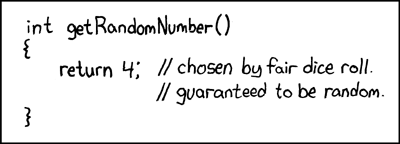
\includegraphics[scale=0.6]{xkcd/random_number}
				\vspace{-7pt}
				\caption{ \texttt{\url{http://xkcd.com/}} }
			\end{figure} 	
		}
	\end{block}
\end{frame}

%% Zum Aufwärmen

\begin{frame}{Der Philosoph am Scheideweg}
	\only<1|handout:1>{
	Ein Weg führt in die Wüste, auf dem ein Wanderer marschiert. 
	Nach einem eintägigen Fußmarsch gelangt er an eine Weggabelung, an der eine kleine Hütte steht.\\
	\bigskip
	Neben der Eingangstüre ist ein Plakat mit folgendem Text befestigt:
	}
	\only<2|handout:1>{
		Einer der beiden weiterführenden Wege führt zu mehreren guten Oasen; nur auf diesem Weg kannst du dein Ziel lebend erreichen.\\
		\bigskip
		Der andere Weg führt in die unendliche Wüste; er hat noch jedem den Tod gebracht, der ihn wählte.\\
		\bigskip
	}
	\only<2-3|handout:2>{
		In dieser Hütte haust ein Philosoph, der die Ziele der beiden Wege sicher kennt; \textbf{streng abwechselnd sagt er an einem Tag die Wahrheit und am darauf folgenden Tag lügt er}.\\
		\bigskip
		Keiner außer ihm weiß aber, ob der heute die Wahrheit sagt oder aber heute lügt.\\
		\bigskip
	}
	\only<3|handout:2>{
		Du darfst dem Philosophen nur eine einzige Frage stellen, mit der du den Weg zu den Oasen erfahren willst.\\
		\bigskip
		Was fragst du ihn?
	}
\end{frame}

\begin{frame}{Der Philosoph am Scheideweg}
	Was fragst du ihn?\\[1em] \pause
	Was würdest du sagen, wenn ich dich morgen fragen würde, ob der linke Weg der richtige ist?\\
	\bigskip
	Und wenn der Philosoph jeden Morgen würfelt, ob er die Wahrheit sagt oder lügt?\\ 
	\only<2|handout:2>{
		Was würdest du sagen, wenn ich dich \textbf{heute} fragen würde, ob der linke Weg der richtige ist?\\
	}
\end{frame}

\section{Relationen}
\begin{frame}{Eigenschaften}
	\begin{Definition}
		Sei $R \subseteq A \times A$ eine (binäre) Relation auf der Menge $A$. Wir nennen $R$
		\begin{itemize}[<+->]
			\item \textbf{reflexiv} falls gilt $$\forall x \in A: (x,x) \in R$$
			\item \textbf{symmetrisch} falls gilt $$\forall x,y \in A: (x,y) \in R \implies (y,x) \in R$$
			\item \textbf{transitiv} falls gilt $$\forall x,y,z \in A: (x,y) \in R \text{ und } (y,z) \in R \implies (x,z) \in R$$
		\end{itemize}
	\end{Definition}
\end{frame}

\begin{frame}{Beispiele}
	\begin{itemize}
		\item Die Relation $=$ ist \pause reflexiv, symmetrisch und transitiv. Man nennt so etwas auch Äquivalenzrelation
		\item \pause Die Relation $<$ ist \pause nicht reflexiv und nicht symmetrisch, aber transitiv
		\item \pause Die Relation $\leq$ ist \pause reflexiv, nicht symmetrisch, aber transitiv
	\end{itemize}
\end{frame}

\begin{frame}{Produkt}
	\begin{Definition}
		Das \textbf{Produkt} von zwei Relationen $R \subseteq M \times N, S \subseteq N \times L$ definieren wir als $$S \circ R = \{(x,z) \in M \times L \mid \exists y \in N \ : \ (x,y) \in R \text{ und } (y,z) \in S \}$$
	\end{Definition}	
	\pause
	
	\begin{Definition}
		Die \textbf{Potenz} einer Relation $R \subseteq M \times M$ definieren wir als
		\begin{align*}
			R^0 &= I_M = \{(x,x) \mid x \in M \} \\
			R^{i+1} &= R^i \circ R
		\end{align*}
	\end{Definition}

	\pause
	\begin{block}{Beobachtung}
		Wenn $f$ und $g$ Funktionen sind (also linkstotale, rechtseindeutige Relationen), entspricht $f \circ g$ der Hintereinanderausführung von $f$ nach $g$.
	\end{block}
\end{frame}

\begin{frame}{Reflexiv-transitive Hülle}
	\begin{Definition}
		Die \textbf{reflexiv-transitive Hülle} einer Relation $R$ ist
		$$R^\ast = \bigcup \limits_{i=0}^\infty R^i$$
	\end{Definition}

	\pause
	\begin{block}{Satz}
		$R^*$ ist die kleinste Relation, die $R$ umfasst und reflexiv und
		transitiv ist.
	\end{block}

	\pause
	\begin{Beispiel}
		Sei $A = \{a, b, c, d, e\}$ und R = $\{(a, b), (b, c), (c, e)\} \subseteq A \times A$\\ \pause
		%TODO Align
		$R^*=\{(a,a), (b,b), (c,c), (d,d), (e,e),$ \\
		$(a,b), (b,c), (c,e),$ \\
		$(a,c), (b,e),(a,e)\}$
	\end{Beispiel}
	
\end{frame}




\begin{frame}{Noch offen: Klammerausdrücke}
	A long, long time ago, in a land far away:\\
	Formale Sprachen angeben durch Mengen, Konkatenation und Kleenschem Abschluss...\\
	Was ist mit der Sprache aller gültigen Klammerausdrücke? Können wir diese auch auf diese Weise angeben?\\[1em]
	\pause
	Jetzt wissen wir: Nein, das geht nicht! (Siehe VL)\\[1em]
	
	\begin{figure}[H]
		\centering
		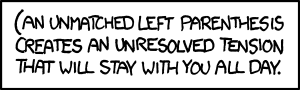
\includegraphics[scale=0.7]{xkcd/(.png}
		\vspace{-7pt}
		\caption{ \texttt{\url{https://xkcd.com/859/}} }
	\end{figure}
\end{frame}

\section{Kontextfreie Grammatiken}
\begin{frame}{Kontextfreie Grammatiken}
	
	\begin{Definition}
		Eine \textbf{kontextfreie Grammatik} ist ein 4-Tupel $G = (N, T, S ,P)$ mit
		\begin{itemize}
			\item[$N$] Alphabet von Nichtterminalsymbolen
			\item[$T$] Alphabet von Terminalsymbolen ($N \cap T = \emptyset$)
			\item[$S$] Startsymbol ($S \in N$)
			\item[$P$] Produktionsmenge ($P \subseteq N \times (N \cup T)^\ast$)
		\end{itemize}
	\end{Definition}

	\pause
	\begin{Beispiel}
		Sei $A$ das deutsche Alphabet (mit Klein-/Großbuchstaben).\\
		$G_{MI} := \left(\{S, M, I, N\}, \, A \cup \N_+, \, S, \, P\right)$ mit
		\begin{align*}
			P = \{S &\to \text{M\word\sp I\word\sp N}, \\
			M &\to \word{Monkey}, \\
			I &\to \word{Island}, \\
			N &\to \word 1 \mid \word 2 \mid \word 3 \}
		\end{align*}
	\end{Beispiel}
\end{frame}

\begin{frame}{Kontextfreie Grammatiken}
	\begin{block}{Produktionen}
		$=$ Menge von Ersetzungsregeln. \\
		Schema: \\
		\qqquad $\underbrace{L}_{\mathclap{\text{\textbf{genau ein} Nichtterminal}}} \to [\text{rechte Seite aus \word{Terminalen} und/oder Nichtterminalen}]$ \\
		\smallskip
		Heißt: Wir können in \textbf{einem} Ersetzungsschritt \textbf{genau ein} solches Nichtterminal $L$ mit der rechten Seite ersetzen. \textbf{Wenn wir wollen}. \\
		\medskip
		\pause
		Mehrere Möglichkeiten zur Auswahl: \\
		\qquad $L \to [\text{rechte Seite}]_1 \mid [\text{rechte Seite}]_2 \mid [\text{rechte Seite}]_3 \mid ...$ \\
		Heißt: $L$ kann durch die rechte Seite 1, 2 oder 3 ersetzt werden. \textbf{Wie wir wollen.} \\
		\pause
		\begin{Beispiel}
			$S \to \word aB\word x \mid \word{zz}$ \\
			\impl $S$ kann durch $\word aB\word x$ oder \word{zz} ersetzt werden.
		\end{Beispiel}
	\end{block}
\end{frame}

\begin{frame}{Ableitungen von Wörtern}
	\begin{Definition}
		Wort $u = .....X.....$ \textbf{ableitbar} nach $v = ..... w......$ \\
		wenn es eine Produktion $X \to w$ gibt. \; ($X$ ist Nichtterminal.) \\
		Schreibweise: \quad $u \derives v$ \quad oder \quad $u \derives^1 v$ \\
	\end{Definition}
	
	\medskip
	\textbf{\alert{Achtung}}: Aufpassen mit Pfeilen: \quad  $\derives$ vs. $\to$
	
	\pause
	\begin{Beispiel}
		Für $G_{MI}$ gilt: \\
		$S \derives M\word{\sp} I\word{\sp}N$\\
		$ M\word{\sp} I\word{\sp}N \derives \word{Monkey}\word{\sp} I\word{\sp} N \derives \word{Monkey}\word{\sp} I\word{\sp 3}$ \\
		$\word{Monkey}\word{\sp} I\word{\sp} N \derives \word{Monkey}\word{\sp} I\word{\sp 1} \derives \word{Monkey}\word{\sp}\word{Island}\word{\sp 1}$ \\
		Es gibt kein Wort, das aus \word{Monkey\sp Island\sp 1} abgeleitet werden kann.
	\end{Beispiel}
	
\end{frame}

\begin{frame}{Ableitung}	
	\begin{block}{Schreibweisen}
		$u \derives^k v$ \quad heißt: $u$ in $k$ Schritten ableitbar zu $v$ \\
		$u \derives^0 v$ \quad heißt also: in 0 Schritten ableitbar ($u=v$) \\
		\smallskip
		$u \derives^* v$ \quad heißt: $u$ in \emph{beliebig vielen} Schritten ableitbar zu $v$
	\end{block}
	
	\mycomment{
		\pause
		\begin{block}{Beobachtung}
			Die Definitionen stimmen mit den Potenzen der Relation $\derives$ überein.\\
			$\derives^\ast$ ist die reflexiv-transitive Hülle von $\derives$.
		\end{block}
	}
	
	\pause
	\begin{Beispiel}
		Für $G_{MI}$ gilt: $S \derives^3 \word{Monkey\sp Island\sp}N \derives^1 \word{Monkey\sp Island\sp3}$\\
		$S \derives^* \word{Monkey\sp Island\sp2}$
	\end{Beispiel}
\end{frame}


\begin{frame}{Erzeugte Sprache einer Grammatik}
	\begin{Definition}
		Sei $G = (N, T, S, P)$ eine kontextfreie Grammatik. Wir nennen die Sprache $$L(G) := \{w \in T^\ast \mid S \Rightarrow^\ast w \} \subseteq T^*$$ die von $G$ \textbf{erzeugte Sprache}.
	\end{Definition} \pause
	Das sind also alle Wörter aus \emph{Terminalsymbolen}, die vom Startsymbol aus ableitbar sind.\\
	\bigskip
	Achtung: Die erzeugte Sprache kann auch \textbf{leer} sein. \\
	\§{Beispiele:} \pause $L\left(\left(\{X\},\, \{\word a, \word b\},\, X\, ,\{X\to X\}\right)\right) = \emptyset$ \pause \quad oder \\
	\. $L\left(\left(\{X\},\, \{\word a, \word b\},\, X\, ,\emptyset \right)\right) = \emptyset$
\end{frame}

\begin{frame}{Erzeugte Sprache}
	\begin{Beispiel}
		$L(G_{MI}) = \{\word{Monkey\sp Island\sp1}, \word{Monkey\sp Island\sp 2}, \word{Monkey\sp Island\sp 3}\}$\\
		$M\wordsp I\wordsp N \notin L(G_{MI})$ \quad (enthält nämlich  Nichtterminale!)
	\end{Beispiel}
	
	\pause
	\begin{Definition}
		Eine Sprache $L$, für die irgendeine kontextfreie Grammatik G mit $L(G) = L$ existiert, heißt \textbf{kontextfrei}.
	\end{Definition}
	\medskip
	
	Viele Programmiersprachen sind kontextfrei. \\ 
	% Fun fact: Einrücksensitive Sprachen (wie Python – oder Haskell <3) sind dies streng genommen nicht! Das Lexing kann dann nicht von einem Regex-Automaten gemacht werden, der („übermächtige“ Stack-Automaten-)Lexer muss dann den Input vorverarbeiten, der daraus entstehende Tokenstream kann dann kontextfrei geparst werden.  Source: http://trevorjim.com/python-is-not-context-free/
	Eine vereinfachte Variante der englischen Sprache auch. \smiley
% Grob falsch:
%	Viele \enquote{natürlich vorkommende} Sprachen sind kontextfrei.
		
\end{frame}

\subsection{Beispiele}
\begin{frame}{Beispiel}
	$$ G = (\{X\}, \, \{\word a, \word  b\}, \, X, \, \{X \to \word aX\word b \mid \eps\}) $$
	\delimitershortfall=1pt
	\begin{itemize}
		\item Gilt $X \derives \word aX\word b$, \; $X \derives \word{aa}X\word{bb}$, \; $XX \derives \word{a}X\word{ba}X\word{b}$? \\
			  \visible<2-|handout:2->{Ja, Nein, Nein.}
		\item Welche Wörter über $\{\word a, \word  b\}$ lassen sich aus $\word{aa}X\word{bb}$ ableiten? Und aus $XX$? \\
			  \visible<3-|handout:2->{
				  Aus $\word{aa}X\word{bb}$: \quad $\set{\word a^k\word b^k \mid k \geq 2}$ \\
				  Aus $XX$: \quad $\set{\word a^k\word b^k \word a^\ell \word b^\ell \mid k,\ell \in \N_0}$
			  }
		\item Gebt $L(G)$ an! \\
		      \visible<4-|handout:2->{ $L(G) = \set{\word a^k\word b^k\mid k \in \N_0}$ }
	\end{itemize}
	
\end{frame}

\begin{frame}{Klammerausdrücke}
	Gegeben sei die Grammatik $$G = (\{X\}, \{\word{(}, \word)\}, X, \{X \to XX \mid \word(X\word) \mid \eps\})$$
	\begin{itemize}
		\item Wie leitet man \word{(())} ab?
		\item Wie leitet man \word{()()} ab?
		\item Kann man \word{(()(} ableiten? \pause \impl Nein!
		\item Und wie leitet man \word{(())()()} ab?\\ \pause
			$X \derives XX \derives XXX \derives \word(X\word)XX \derives \word(X\word)X\word(X\word) \derives \word(X\word)\word(X\word)\word(X\word)$ \\
			$\quad \derives \word(X\word{)()(}X\word) \derives \word{((}X\word{))()(}X\word) \derives \word{((}X\word{))()()} \derives \word{(())()()}$\\
			Geht das auch übersichtlicher? \impl Ableitungsbäume
	\end{itemize}
\end{frame}


\begin{frame}{Ableitungsbäume}
	\centering
	$G = (\{X\}, \{\word{(}, \word)\}, X, \{X \to XX \mid \word(X\word) \mid \eps\})$
	\medskip
	
	\begin{tikzpicture}
	[level 1/.style={sibling distance=50mm},
	level 2/.style={sibling distance=30mm},
	level 3/.style={sibling distance=10mm}]
	\node {$X$}
	child { node {$X$}
		[level 2/.style={sibling distance=15mm}]
		child {node {$\literal{(}$} }
		child {node {$X$} 
			child {node {$\literal{(}$} }
			child {node {$X$}
				child {node {$\varepsilon$} }
			}
			child {node {$\literal{)}$} }
		}
		child {node {$\literal{)}$} }
	} 
	child { node {$X$} 
		child { node {$X$} 
			child {node {$\literal{(}$} }
			child {node {$X$}
				child {node {$\varepsilon$} }
			}
			child {node {$\literal{)}$} }
		}
		child { node {$X$} 
			child {node {$\literal{(}$} }
			child {node {$X$}
				child {node {$\varepsilon$} }
			}
			child {node {$\literal{)}$} }
		}
	} ;
	\end{tikzpicture}
\end{frame}


\begin{frame}{Klammerausdrücke}
	Gegeben sei die Grammatik $$G = (\{X\}, \{\word{(}, \word)\}, X, \{X \to XX \mid \word(X\word) \mid \eps\})$$
	Was ist $L(G)$? Was kann man also aus $X$ ableiten?\\ \pause 
	Alle \enquote{\textit{wohlgeformten Klammerausdrücke}} \quad ($=$ alle, die Sinn machen).\\[1em]
	
	Was bedeutet wohlgeformt in diesem Kontext?\\ \pause
	$$\forall w \in L(G): N_{\word(}(w) = N_{\word)}(w)$$ 
	Reicht das? \pause \impl Notwendig, aber nicht hinreichend! 

\end{frame}

\begin{frame}{Klammerausdrücke}
	Wir dürfen eine Klammer erst schließen, \textit{nachdem} wir sie geöffnet haben.\\
	Also: Anzahl der schließenden Klammern darf nie größer als Anzahl der öffnenden Klammern sein! \pause \\[1em]
	\impl Für jedes Präfix $v$ von einem Wort $w \in L(G)$ gilt $$N_{\word(} (v) \geq N_{\word)} (v)$$ \pause
	
	\textbf{Achtung}: Grammatiken sind \textbf{nicht eindeutig}! Wir können zur gleichen Sprache mehrere verschiedene erzeugende Grammatiken finden. \\
	Alternative Grammatik für wohlgeformte Klammerausdrücke: \pause $$G = (\{X\}, \, \{\word (, \word )\}, \, X, \, \{X \to \word(X\word)X \mid \varepsilon\})$$
\end{frame}

\begin{frame}{Und jetzt ihr...}
	Gebt jeweils eine Grammatik über dem Alphabet $T = \{\word a, \word b\}$ an, die folgende Sprache erzeugt:
	\begin{itemize}
		\item Alle Wörter, in denen irgendwo das Teilwort $\word{baa}$ vorkommt.\\
		\visible<2-|handout:2>{
			$(\{X,Y\},T,X,P)$ mit $P=\{X \to Y\word{baa}Y, Y \to \word aY \mid \word bY \mid \varepsilon\}$
		}
		
		\item Alle Wörter, in denen $\word{ab}$ als Teilwort vorkommt oder kein $\word a$ enthalten ist. \\
		\visible<3-|handout:2>{
			$G = (\{X, Y\}, \{\word a, \word b\}, X, P)$ mit $P = \{X \to \word bX \mid Y\word{ab}Y \mid \varepsilon, Y \to \word aY \mid \word bY \mid \varepsilon\}$
		}
		
		\item Die Menge aller Wörter $w\in T^*$ mit der Eigenschaft, dass
		für alle Präfixe $v$ von $w$ gilt: $\setsize{N_{\word{a}}(v) - N_{\word{b}}(v)} \leq
		1$.\\
		\emph{Tipp}: Was für eine Struktur haben Wörter der Länge $2$, $4$, \dots? \\
		% $\{ab, ba\}^*$
		\visible<4-|handout:2>{
			$(\{X,Y\},T,X,P)$ mit $P=\{X \to \word{ab}X \mid \word{ba}X \mid \word a \mid \word b \mid \varepsilon\}$
		}
		
	\end{itemize}
\end{frame}


\begin{frame}{Aufgabe: Palindrome}
	\begin{itemize}
		\item Geben Sie eine kontextfreie Grammatik $$G = (N, \{\word a, \word b\}, S, P )$$ an, für die $L(G)$ die Menge aller Palindrome über dem Alphabet $\{\word a, \word b\}$ ist.
		\item Geben Sie eine Ableitung der Wörter \word{baaab} und \word{abaaaba} aus dem Startsymbol Ihrer Grammatik an.
		\item Beweisen Sie, dass Ihre Grammatik jedes Palindrom über dem Alphabet $\{\word a, \word b\}$ erzeugt.\\
		(\emph{Tipp}: Induktion: Wenn's für $n$ und $n+1$ gilt, dann gilt's auch für $n+2$.)
	\end{itemize}
\end{frame}

\begin{frame}{Lösung}
	Die Grammatik $$G = (\{S\}, \{\word a, \word b\}, S, P = \{S \to \word aS\word a \ | \ \word bS\word b \ | \ \word a \ | \ \word b \ | \ \varepsilon \})$$ erzeugt gerade die Menge der Palindrome. \pause Die Ableitungen der Wörter mit dieser Grammatik sind 
	$$S \derives \word bS\word b \derives \word{ba}S\word{ab} \derives \word{baaab}$$
	$$S \derives \word aS\word a \derives \word{ab}S\word{ba} \derives \word{aba}S\word{aba} \derives \word{abaaaba}$$
\end{frame}

\begin{frame}{Lösung}
	Sei $w$ ein Palindrom über $\{\word a,\word b\}$. Wir zeigen durch Induktion über $n = \size{w}$, dass alle Palindrome aus $S$ abgeleitet werden können. \pause
	\begin{block}{Induktionsanfang} \pause
		Für $n = 0$ ist das leere Wort $\varepsilon$ in einem Schritt aus $S$ ableitbar. \\
		Für $n=1$: Die einzigen Wörter aus $\{\word a,\word b\}^\ast$ der Länge 1 sind $\word a$ und $\word b$. Auch diese sind offensichtlich aus $S$ ableitbar.
	\end{block}
 	\pause
	\begin{block}{Induktionsvoraussetzung} \pause
		Für ein festes, aber beliebiges $n \in \N_0$ gilt, dass alle Palindrome der Länge $n$ und alle Palindrome der Länge $n + 1$ aus S abgeleitet werden können.
	\end{block}
\end{frame}

\begin{frame}{Lösung}
		\begin{block}{Induktionsschritt}
			Sei $w$ ein Palindrom der Länge $n + 2$. Das erste (und damit auch das letzte) Zeichen sei oBdA. ein $\word a$. Dann gibt es ein $w' \in \{\word a, \word b\}^\ast$, so dass $w = \word aw'\word a$ ist. Da $w$ ein Palindrom ist, muss auch $w'$ ein Palindrom sein. Weiterhin gilt $\size{w'} = n$. \pause Nach IV gibt es somit eine Ableitung $S \derives^\ast w'$. Somit gibt es die Ableitung $$S \derives \word aS\word a \overset{IV}{\derives^\ast} \word aw'\word a = w$$ und $w \in L(G)$ folgt. \pause Entsprechendes gilt, wenn das erste Zeichen von w ein \word b ist. \\
			Mit der IV haben wir also gezeigt, dass auch Palindrome der Länge $n+1$ und $n+2$ aus $S$ ableitbar sind.
	\end{block}

\end{frame}

\begin{frame}{Gibt es noch mehr?}
	Viele Sprachen in der Informatik sind kontextfrei.\\[1em]
	Was ist mit der Sprache $L_{vv} = \{v\word cv \mid v \in \{\word a,\word b\}^*\}$\\
	\smallskip
	\pause
	In der Vorlesung: Es gibt keine kontextfreie Grammatik, die $L_{vv}$ erzeugt.\\
	\medskip
	\pause
	Können wir die Sprache trotzdem irgendwie \enquote{verarbeiten}?
	
	\begin{block}{}
		\Large
		\centering
		Soon...\\[1em]
	\end{block}
\end{frame}



\begin{frame}	
	\begin{block}{Was ihr nun wissen solltet}
		\begin{itemize}
			\item Mehr Eigenschaften von Relationen
			\item Was eine kontextfreie Grammatik ist
			\item Wie man Sprachen aus Grammatiken ableiten kann
		\end{itemize}
	\end{block}
	
	\begin{block}{Was nächstes Mal kommt}
		\begin{itemize}
			\item Nachts sind alle Katzen grau - Prädikatenlogik
			\item Algorithmen: Kochrezepte der Informatik
		\end{itemize}
	\end{block}
\end{frame}

\lastframe{0.50}{0}{xkcd/exploits_of_a_mom.png}{https://www.xkcd.com/327/}
\slideThanks

\end{document}